\begin{frame}
\frametitle{Key Points}
\begin{itemize}
\item Why we search for good, but not always optimal solutions
\item The different objectives provided in scheduling tool
\item More complex optimization schemes involving multiple objectives
\item Other criteria that might guide which solution we prefer
\item An interesting research direction
\end{itemize}
\end{frame}

\section{Optimal vs. Good Solutions}

\begin{frame}
\frametitle{Why have an Objective?}
\begin{itemize}
\item For most scheduling problem, we define some form objective
\item A mathematical formula that we evaluate on a schedule to compare it
\item It is not always clear whether that formula represents some direct business benefit
\item But, there are far more bad solutions than good solutions!
\item The objective tells us if the solution is more "good" or "bad"
\item Different stakeholders will have different views what makes a solution "good" or even "acceptable"
\end{itemize}
\end{frame}

\begin{frame}
\frametitle{Minimizing Cost vs Maximizing Profit}
\begin{itemize}
\item A lot of objectives aim to reduce cost of production
\item This is not always a good thing
\begin{itemize}
\item Doing nothing costs nothing
\end{itemize}
\item But defining the profit obtained by a schedule is not easy
\item Many intangible factors weigh in
\begin{itemize}
\item Happiness of the customers (which customers are unhappy, does it matter?)
\item Happiness of personnel (finding and retaining skilled personnel is critical)
\item Happiness of stakeholders (sales, production, inventory, management)
\end{itemize}

\end{itemize}
\end{frame}

\begin{frame}
\frametitle{Timeliness}
\begin{itemize}
\item How quickly do we need a solution?
\begin{itemize}
\item Sometimes we need a solution right now
\item We may also have time to wait a bit, or even more
\item Waiting five minutes, having a short break for a coffee, will often be acceptable
\item For some problems, running a scheduler overnight is possible
\item Do we need the ultimate in solution quality, or an acceptable solution right now? 
\end{itemize}
\item Benchmarks are often run with unlimited resources
\begin{itemize}
\item "We used four years of computer time to solve these problems"
\end{itemize}
 
\end{itemize}
\end{frame}

\begin{frame}
\frametitle{Diminishing Returns Running a Solver}
\includegraphics[width=\textwidth]{../05-objectives/images/intermediate-solutions}

\begin{itemize}
\item Which compromise between quality and speed are we looking for?
\end{itemize}

\end{frame}









\subsection{Cost vs. Profit Based Objectives}

\section{Objective Types}

\begin{frame}
\frametitle{Setting the Objective}
\begin{columns}
\begin{column}{0.6\textwidth}
\begin{itemize}
\item We can select a predefined objective in solver dialog
\item There are weight factors to give more impact to some cost terms in on-time and hybrid objectives
\end{itemize}
\end{column}
\begin{column}{0.4\textwidth}
\includegraphics[width=\textwidth]{../05-objectives/images/setting-objective}
\end{column}
\end{columns}
\end{frame}


\subsection{Makespan}

\begin{frame}
\frametitle{Makespan \avail}
\includegraphics[width=.8\textwidth]{../05-objectives/images/objective-makespan}

\begin{itemize}
\item Minimize the overall project end
\item Very traditional objective in scheduling
\begin{itemize}
\item Justified in project scheduling
\item Not so clearly justified in manufacturing
\end{itemize}
\item A number of jobs are significantly late

\end{itemize}
\end{frame}


\subsection{Flowtime}
\begin{frame}
\frametitle{Flowtime \avail}
\includegraphics[width=.8\textwidth]{../05-objectives/images/objective-flowtime}

\begin{itemize}
\item Minimize the sum of job ends
\item Prefer any machine to end early
\item Not always easy to find good solutions
\end{itemize}
\end{frame}

\subsection{Lateness}

\begin{frame}
\frametitle{Total Lateness \avail}
\includegraphics[width=.8\textwidth]{../05-objectives/images/objective-totallateness}

\begin{itemize}
\item Able to remove all delays on jobs
\item Does not care about makespan or earliness

\end{itemize}
\end{frame}


\subsection{On-Time}
\begin{frame}
\frametitle{Maximizing On-Time Delivery \avail}
\includegraphics[width=.8\textwidth]{../05-objectives/images/objective-ontime}

\begin{itemize}
\item Weight 100 for lateness, weight 1 for earliness
\item Removes all delays, very little earliness
\item Makespan increased dramatically

\end{itemize}
\end{frame}


\subsection{Hybrid}

\begin{frame}
\frametitle{Hybrid Objective \avail}
\includegraphics[width=.8\textwidth]{../05-objectives/images/objective-hybrid}

\begin{itemize}
\item Weights makespan:1000, flowtime:0, lateness:10, earliness:1
\item Does not remove lateness completely
\item Probably needs more time to improve
\end{itemize}
\end{frame}

\begin{frame}
\frametitle{Hybrid Objective (Enforce Duedate)\avail}
\includegraphics[width=.8\textwidth]{../05-objectives/images/objective-hybrid-enforce-duedate}

\begin{itemize}
\item Sometimes enforcing a constraint is more powerful
\item Here require that due dates are respected
\item Leads to overall better solution
\end{itemize}
\end{frame}

\subsection{Comparison}

\begin{frame}
\frametitle{Comparing Solutions with Different Objectives}
\includegraphics[width=\textwidth]{../05-objectives/images/compare-solutions}
\begin{itemize}
\item System tries to reduce the objective
\item May mean other aspect of solution is poor
\begin{itemize}
\item \emph{Total Lateness} bad if just reducing \emph{Makespan}
\item \emph{Makespan} bad if just reducing \emph{Total Lateness}
\end{itemize}
\item Hybrid objectives can find better compromises
\item Using constraints to restrict search can help 
\item Needs more work on lower bounds
\end{itemize}

\end{frame}




\subsection{Resource Levels}

\begin{frame}
\frametitle{Optimizing Resource Levels \navail}
\begin{itemize}
\item We have already discussed this in the Resources section
\item Sometimes we aim to optimize resource use, not time or delay
\item Typical is minimizing
\begin{itemize}
\item The number of disjunctive machines needed
\item A cumulative resource capacity
\item The manpower required to perform all tasks
\end{itemize}
\item We may do this for understanding the problem
\item The optimized schedules will be brittle
\begin{itemize}
\item Any resource breakdown will cause an issue
\item Spare capacity is a good thing (if it is not too expensive)
\end{itemize}

\end{itemize}
\end{frame}

\begin{frame}
\frametitle{Multi-level Objectives \navail}
\begin{itemize}
\item In some situations, a hybrid objective combining different aspects is not enough
\item We need to find the best compromises between the different objective types
\begin{itemize}
\item Without an a-priori weight to state which is more important
\end{itemize}
\item A solution \emph{dominates} another solution, if for all objective types, it is better than the other
\item Two solutions are \emph{incomparable} if for some objective type one solution is better, but for some other objective, the other solution is better
\item \emph{Pareto frontier}: Set of all non-dominated, incomparable solutions
\end{itemize}
\end{frame}

\begin{frame}
\frametitle{Pareto Frontier for Two Incomparable Objectives}
\scalebox{0.5}{
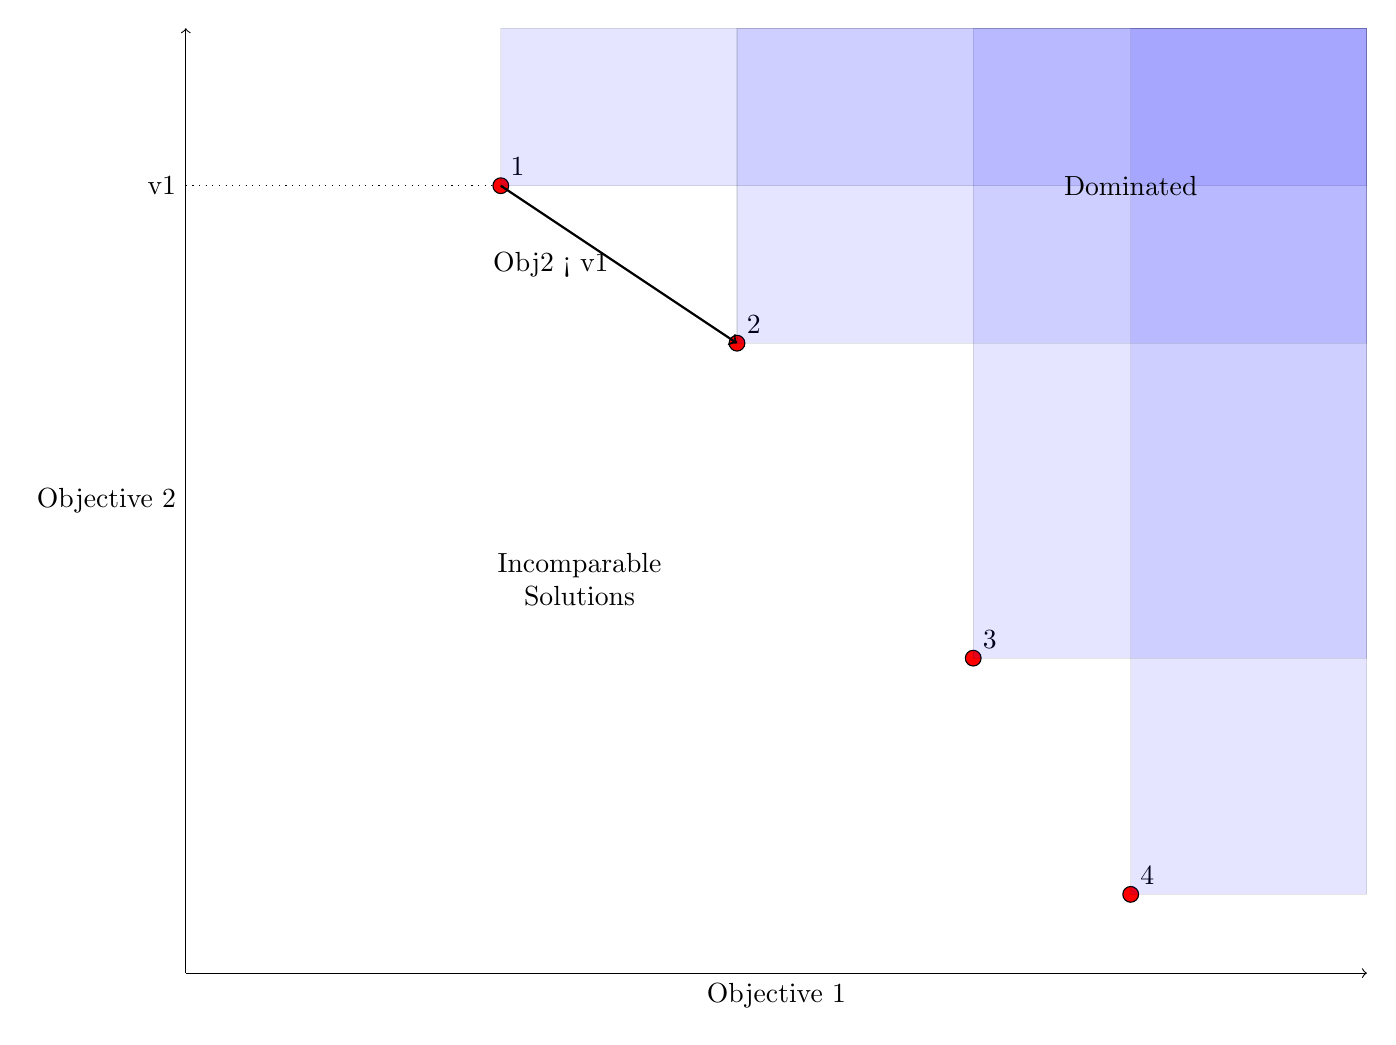
\begin{tikzpicture}
\draw[black,->] (0,0) -- node[below]{Objective 1} (15,0);
\draw[black,->] (0,0) -- node[left] {Objective 2} (0,12);
\node[left] at (0,10) {v1};
\draw[dotted] (0,10) -- (4,10);
\draw[fill=red] (4,10) circle (0.1) node[above right]{1};
\draw[fill=red] (7,8) circle (0.1) node[above right]{2};
\draw[fill=red] (10,4) circle (0.1) node[above right]{3};
\draw[fill=red] (12,1) circle (0.1) node[above right]{4};
\draw[fill=blue,opacity=0.1] (12,1) rectangle +(3,11);
\draw[fill=blue,opacity=0.1] (10,4) rectangle +(5,8);
\draw[fill=blue,opacity=0.1] (7,8) rectangle +(8,4);
\draw[fill=blue,opacity=0.1] (4,10) rectangle +(11,2);
\node at (12,10) {Dominated};
\node at (5,5) {\shortstack{Incomparable\\Solutions}};
\draw[thick,black, ->] (4,10) -- node[left] {Obj2 < v1} (7,8);
\end{tikzpicture}
}
\begin{itemize}
\item Finding Pareto frontier by repeated optimization of objective1
\end{itemize}

\end{frame}


\section{Other Quality Vectors}

\begin{frame}
\frametitle{Other Quality Vectors}
\begin{itemize}
\item There are other scales on which we may measure whether a solution is "good"
\begin{itemize}
\item Fairness
\item Robustness
\item Product Quality
\item Customer Satisfaction
\item Diversity
\end{itemize}
\end{itemize}
\end{frame}

\begin{frame}
\frametitle{Fairness}
\begin{itemize}
\item Typically involves humans
\item If we assign operators, do we
\begin{itemize}
\item Treat all operators in a fair way?
\item Give effective workers more work
\item Provide opportunities for training and skill development
\item De-risk dependency on key personnel 
\end{itemize}
\item Also, use multiple machines of same type consistently 
\begin{itemize}
\item Balanced
\item Not balanced
\end{itemize}

\end{itemize}
\end{frame}

\begin{frame}
\frametitle{Robustness}
\begin{itemize}
\item By scheduling, we create a plan
\item Often, reality does not follow the plan
\begin{itemize}
\item Unforeseen events, machine breakdowns, sick-leave
\item Delays in raw material delivery, inventory problems
\item Rush orders
\item Small variations in plan execution
\end{itemize}
\item Can we protect the plan against certain types of unplanned events?
\item Is the plan still useful when things change?
\item Or, can we update the plan quickly enough to adapt to changes
\end{itemize}
\end{frame}

\begin{frame}
\frametitle{Product Quality}
\begin{itemize}
\item The tighter the schedule, the more risk there is of cutting corners
\item If we minimize curing times to speed up production, quality may be affected
\item The fastest machine is not always the best in terms of quality, cost
\end{itemize}
\end{frame}

\begin{frame}
\frametitle{Customer Satisfaction}
\begin{itemize}
\item Our objectives for minimizing lateness are lacking context
\item Some customers are more important than others
\item Some orders are more important to the customer than others
\item A phone call by a human can capture more detail than an electronic order form
\item We can adjust our schedule if we know what is important and what is not
\begin{itemize}
\item But where do we get this information?
\item How do we avoid that a customer says "all my orders are critical"
\end{itemize}

\end{itemize}
\end{frame}

\begin{frame}
\frametitle{Diversity}
\begin{itemize}
\item Is it sometimes useful to present different solutions to a user to choose from
\item These solutions should be substantially different to make choice meaningful
\item Unfortunately, solvers often find very similar solutions
\item Typically, there are far too many solution to enumerate them all
\item We can add constraints to ask for the next solution to be quite different from the previous ones
\item Needs good definition to define similarity
\item Hamming distance on machine order a good starting point
\end{itemize}
\end{frame}




\section{Key Performance Indicators}

\begin{frame}
\frametitle{Key Performance Indicators (KPI)}
\begin{itemize}
\item Performance indicators can be computed from a given schedule, and allow to compare different schedules to each other
\item Often, these are business oriented, not process driven
\item There is a difference between an objective and a performance indicator
\begin{itemize}
\item The objective drives the search for a solution
\item The KPI evaluates the quality of a solution, can be totally unrelated to objective
\end{itemize}
\item Ideally, the KPI are expressed in such a way that solutions for different problems can be compared
\begin{itemize}
\item Number of late orders, allows comparison of two solutions of the same problem
\item Percentage of late orders, allows comparison of two different schedules
\end{itemize}
\end{itemize}
\end{frame}

\begin{frame}
\frametitle{KPIs for Sample Solutions}

\begin{itemize}
\item Comparing different solutions of running example with enabling/disabling some constraints
\item Compare \emph{Makespan} to \emph{On-time Delivery} objective
\item There is no \emph{Setup Time} constraint specified for this problem
\end{itemize}

\includegraphics[width=\textwidth]{../05-objectives/images/solutions1}

\includegraphics[width=\textwidth]{../05-objectives/images/solutions2}
\end{frame}

\begin{frame}
\frametitle{KPIs Already Defined \avail}
\begin{description}
\item[Makespan] Max of job ends
\item[Flowtime] Sum of job ends
\item[Total Lateness] Sum of job lateness (tardiness)
\item[Max Lateness] Max of job lateness
\item[NrLate] Number of late jobs
\item[WeightedLateness] Weighted sum of job lateness
\item[PercentLate] percentage of late jobs
\item[...Earliness] same indicators, but for earliness
\item[Duration] Difference between overall start and overall end
\item[Start] start of earliest job
\item[End] end of last job
\end{description}
\end{frame}

\begin{frame}
\frametitle{KPIs Already Defined (cont'd) \avail}
\begin{description}
\item[TotalWait] Sum of Wait time before/after a task of a job
\item[MaxWait] Max wait time before/after a task of a job
\item[TotalIdle] Sum of Idle times of disjunctive machines
\item[MaxIdle] Max Idle Time on a disjunctive machine
\item[TotalSetup] Total setup times
\item[MaxSetup] Max setup time
\item[TotalActiveTime] Total active time between first and last use of a machine
\item[TotalProductionTime] Sum of all task duration
\item[ActiveUtilization] Percentage of production time compared to active time
\item[SetupPercent] Percentage of setup time compared to active time
\item[IdlePercent] Percentage of idle time compared to active time
\end{description}
\end{frame}

\begin{frame}
\frametitle{KPI Ranking \navail}
\begin{itemize}
\item If we have multiple solutions, we want to rank them based on a comparison of different KPIs
\item Different stakeholders will rank different KPIs in very different way
\item This seems to require some customization of the formulas used
\item We can also try to infer a ranking method based on some comparison queries asked to users
\begin{itemize}
\item Do you prefer this or that solution?
\item With enough answers, we can postulate a ranking method
\end{itemize}
\end{itemize}
\end{frame}

\section{Interactive Scheduling}

\begin{frame}
\frametitle{Interactive Scheduling \navail}
\begin{itemize}
\item Some human schedulers are happy to accept a produced plan
\begin{itemize}
\item Perhaps change some constraints, or weights
\end{itemize}
\item Other human schedulers want to modify the plan by hand
\begin{itemize}
\item This is not always easy to do
\item How can a scheduling tool handle this?
\item How much control is given to the user, who checks the constraints?
\item Do we allow the user to create invalid schedules?
\end{itemize}
\end{itemize}
\end{frame}

\begin{frame}
\frametitle{Example: Moses System}
\begin{itemize}
\item Scheduling application for animal feed mills in the UK
\item Produces overnight schedule for delivery on next day
\item Operator updates the schedule whenever a task is finished
\item Change duration of task if it is delayed
\item Move tasks by hand, changing sequence of tasks to be performed
\begin{itemize}
\item System updates constraints, and warns if constraint is violated 
\end{itemize}
\item User can protect part of schedule from modification by system
\begin{itemize}
\item Freeze all tasks up to the selected task
\item Unfreeze the schedule after the selected task
\end{itemize}
\item Related to explainability

\end{itemize}
\end{frame}

\begin{frame}
\frametitle{Screenshot of Moses Application}
\includegraphics[width=\textwidth]{../05-objectives/images/moses}
\end{frame}





\begin{frame}
\frametitle{Summary}
\begin{itemize}
\item Describe the need and role of objectives
\item Presented different objectives available in the scheduling tool
\item Discussed some more advanced possibilities for handling objectives
\item Important to keep user on control of system
\end{itemize}
\end{frame}

